207. \begin{figure}[ht!]
\center{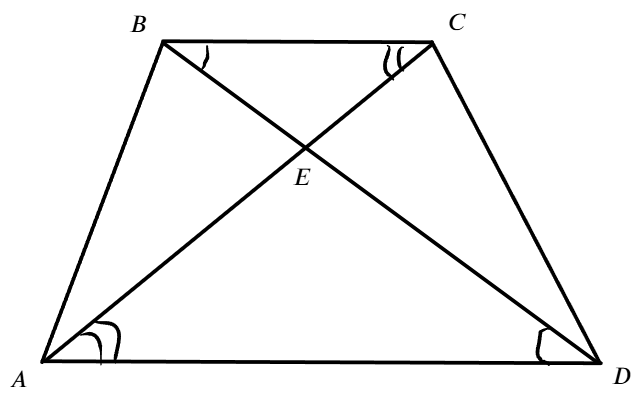
\includegraphics[scale=0.35]{g9-205.png}}
\end{figure}\\
Треугольники $BEC$ и $AED$ подобны по двум углам (накрест лежащим при параллельных прямых $AD$ и $BC$), коэффициент подобия равен $\cfrac{BC}{AD}=
\cfrac{7}{19}.$ Тогда $\cfrac{|BE|}{10-|BE|}=\cfrac{7}{19},\ 19|BE|=70-7|BE|,\ |BE|=\cfrac{35}{13},$ а $\cfrac{|CE|}{24-|CE|}=\cfrac{7}{19},\ 19|CE|=168-7|CE|,\ |BE|=\cfrac{84}{13}.$ Таким образом, в треугольнике $BEC$ имеем равенство $|BE|^2+|CE|^2=\cfrac{1225}{169}+\cfrac{7056}{169}=\cfrac{8281}{169}=49=|BC|^2,$ а значит треугольник $BEC$ является прямоугольным, и угол между прямыми, содержащими диагонали трапеции, равен $90^\circ.$\\
